\documentclass{article}
\usepackage[T1]{fontenc}
\usepackage{graphicx}
\usepackage{float}

\begin{document}

\section{Usługi i aplikacje Internetu Rzeczy - projekt}

\subsection{Kamera z czujnikiem ruchu połączona z aplikacją mobilną}

\paragraph{Aleksander Pajorski, Jan
Narożny}

\subsubsection{1. Raspberry Pi}

\paragraph{1.1 Wymagane elementy}\label{wymagane-elementy}

\begin{itemize}
\item
  Raspberry Pi
\item
  Kompatybilna kamera
\item
  Kompatybilny czujnik ruchu PIR
\end{itemize}

Raspberry Pi powinno być zaktualizowane do najnowszej dystrybucji
Raspbian OS `bookworm'. Należy wykonać

\begin{verbatim}
sudo apt update && sudo apt full-upgrade
\end{verbatim}

aby upewnić się że bibloteki potrzebne do obsługi kamery są dostępne i
aktualne.

\paragraph{1.2 Podłączenie kamery i
czujnika}\label{podux142ux105czenie-kamery-i-czujnika}

Kamerę podączyć~należy przy użyciu dedykowanego kabla oraz portu na
płytce Pi. Kabel musi być dokładnie osadzony, częścią~z kontaktami
skierowany w przeciwnym kierunku niż zatrzask, a sam zatrzask równie
dociśnięty. Czujnik ruchu podłączyć według poniższego schematu:

\begin{figure}[H]
\centering
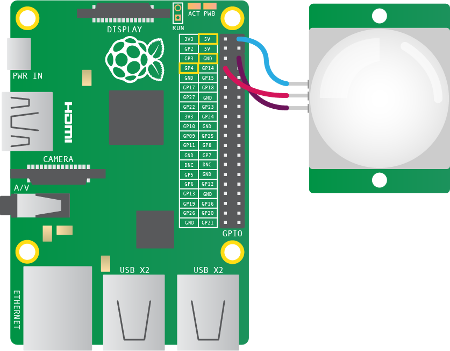
\includegraphics[width=12cm,height=\textheight,keepaspectratio]{images/pir_wiring.png}
\caption{Schemat podłączenia czujnika ruchu}
\end{figure}

Czujnik ruchu posiada 3 piny: Vcc, Gnd, oraz Out. Powinne być one
podpisane. Powyższy schemat jest poglądowy ponieważ~w zależności od
użytej wersji płytki ułożenie pinów GPIO może się~różnić. Pin Vcc na
czujniku podłączyć do pinu zasilającego 5V, pin Gnd do analogcznego pinu
na płytce Pi, a Out do któregokolwiek z pinów GPIO. W tym przypadku
użyty został pin 4. Do przetestowania podłączenia czujnika ruchu:

\paragraph{1.3 Stworzenie python virtual
environment}\label{stworzenie-python-virtual-environment}

\begin{verbatim}
python3 -m venv venv

# windows:
venv\Scripts\activate

# macOS i linux:
source venv/scripts/activate

pip install -r requirements.txt
\end{verbatim}

\paragraph{1.4 Weryfiakcja podłączenia kamery i
czunika}\label{weryfiakcja-podux142ux105czenia-kamery-i-czunika}

Aby zweryfikować poprawne podłączenie czujnika:

\begin{verbatim}
python3 pirTest.py
\end{verbatim}

Zakończyć ctrl+c.~Następnie aby zweryfikować podłączenie kamery:

\begin{verbatim}
rpicam-still -n -o test.jpg
\end{verbatim}

\paragraph{1.5 Chmura azure}\label{chmura-azure}

Zdjęcia przesyłane są do chmury azure, na którym założony został serwis
Azure Blob Storage do przetrzymywania danych. Ze strony głownej Azure
Portal należy wybrać ``Create resource'' i dodać do swojej grupy zasobów
``Storage account''.

\begin{figure}[H]
\centering
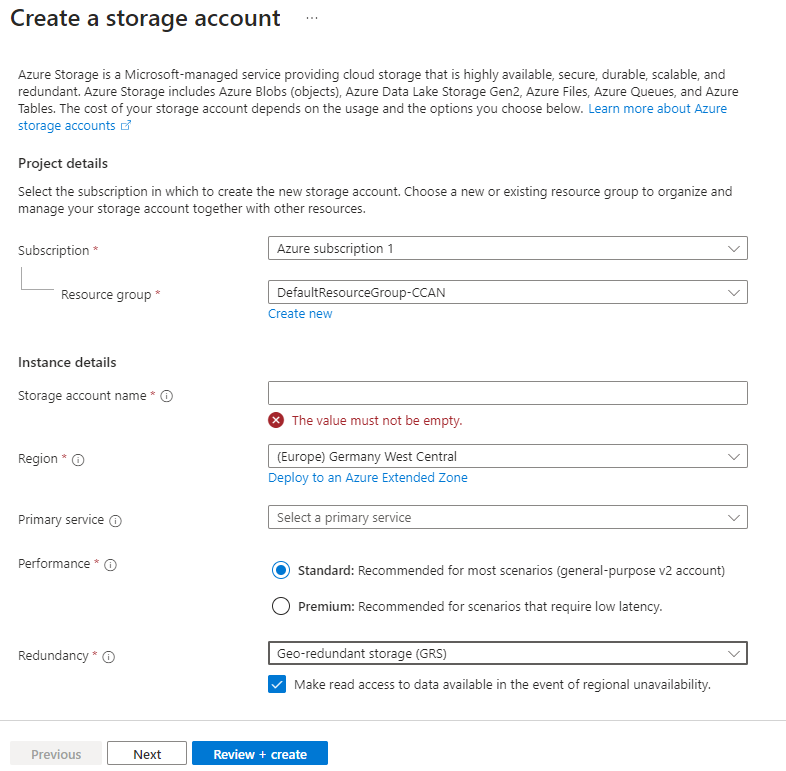
\includegraphics[width=3.125in,height=\textheight,keepaspectratio]{images/create-blob-storage.png}
\caption{Utwórz blob storage}
\end{figure}

W tym miejscu trzeba uzupełnić niezbędne pola: nadać nazwę, wybrać
najbliższy region, primary service może zostać puste, Performance
ustawić na standard a Redundancy na Locally redundant storage dla
najniższych kosztów.

Po utworzeniu tego zasobu należy go otworzyć, z lewego menu wybrać opcję
Containers, i kliknąć opcję dodania kontenera. Opcje zaawansowane na
potrzeby tego projektu są zbędne, więc wystarczy nadać mu nazwę i wybrać
poziom dostępu.

\begin{figure}[H]
\centering
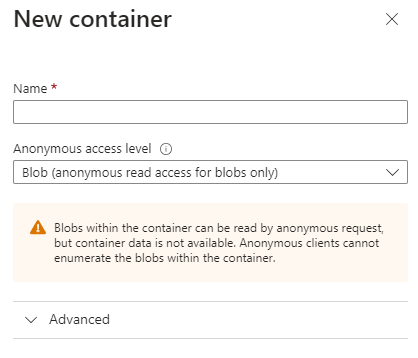
\includegraphics[width=3.125in,height=\textheight,keepaspectratio]{images/container.png}
\caption{Container}
\end{figure}

Następnie należy przejść do ``Access keys'' i pamietać o skopiowaniu
``Connection string'' do kodu na raspberry pi (czy jakimkolwiek innym
urządzeniu, które będzie chciało uzyskać dostęp do tego Blob Storage).

\begin{figure}[H]
\centering
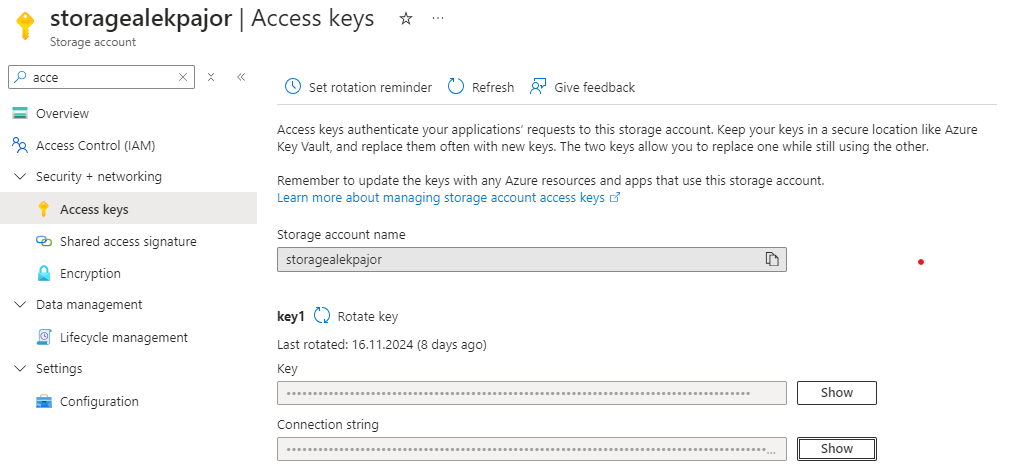
\includegraphics[width=5.20833in,height=\textheight,keepaspectratio]{images/connection-string.png}
\caption{Connection string}
\end{figure}

\paragraph{1.6 Aplikacja mobilna}\label{aplikacja-mobilna}

Aplikacja mobilna napisana została przy użyciu frameworka React Native
oraz Expo w języku TypeScript. PhotoGallery jest głównym komponentem
aplikacji. Po jej otwarciu zdjęcia wczytywane są automatycznie, lecz nie
są automatycznie odświeżane i w przypadku nadejścia nowego zdjęcia
należy ręcznie odświeżyć stronę przesuwając palcem w dół do ukazania się
kółka ładowania. Obok zdjęć znajduje się data oraz godzina ich
utworzenia.

\begin{figure}[H]
\centering
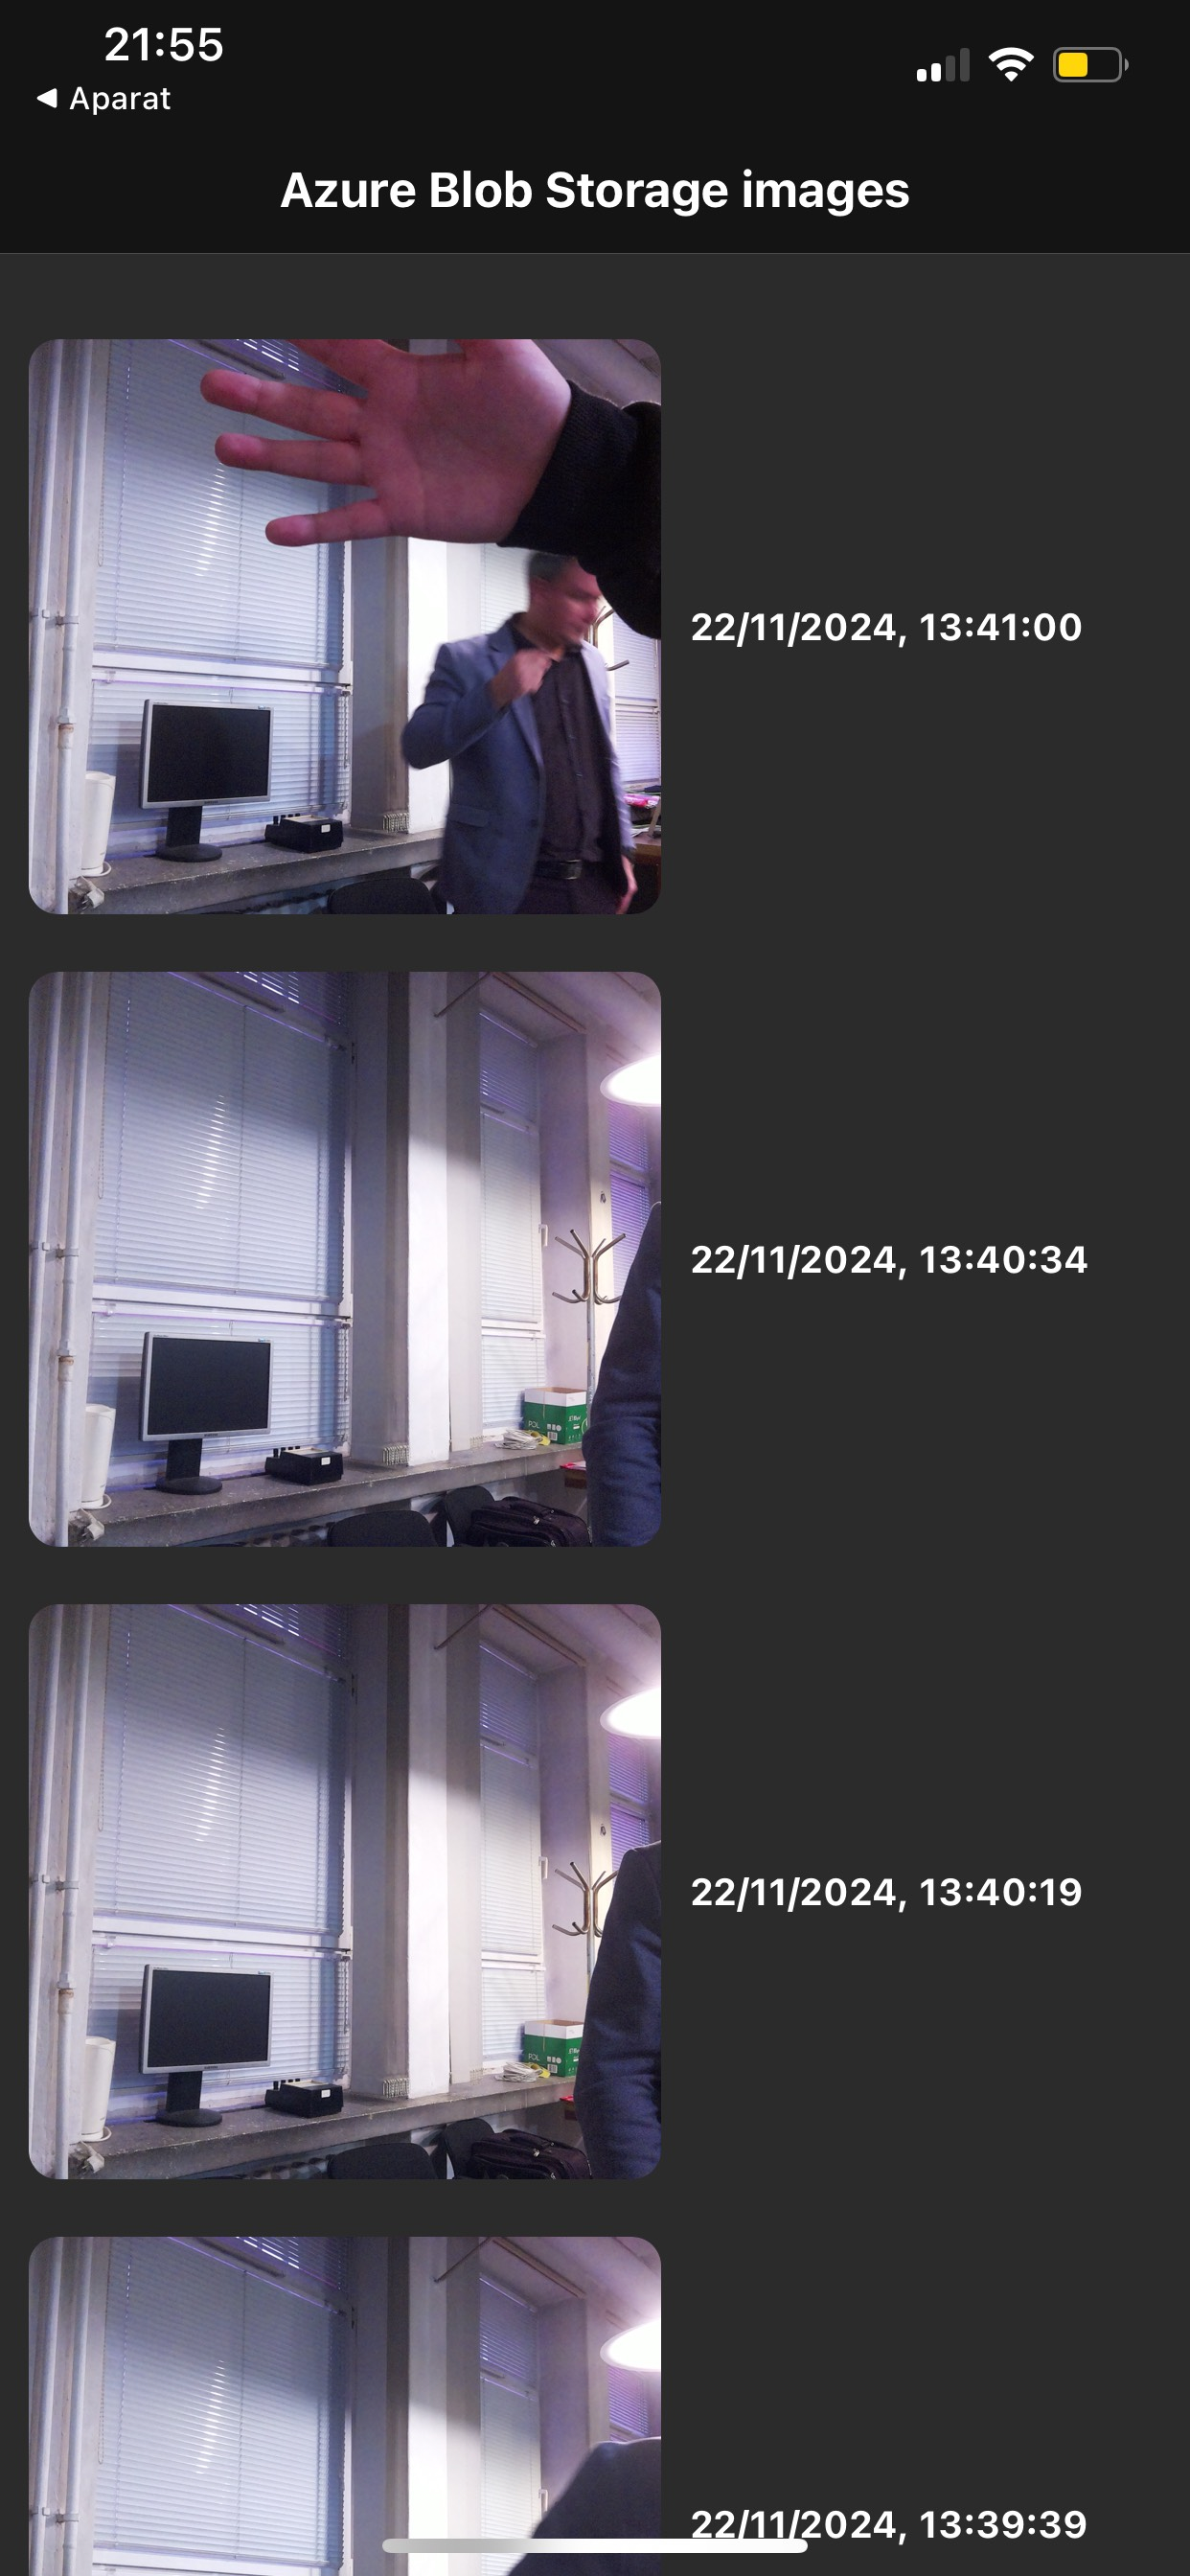
\includegraphics[width=2.60417in,height=\textheight,keepaspectratio]{images/mobile-app.JPG}
\caption{Aplikacja mobilna}
\end{figure}

\begin{verbatim}
import React, { useEffect, useState } from 'react';
import { View, Text, FlatList, Image, ActivityIndicator, StyleSheet } from 'react-native';
import { BlobServiceClient } from '@azure/storage-blob';

const PhotoGallery = () => {
  const [photos, setPhotos] = useState<any[]>([]);
  const [loading, setLoading] = useState<boolean>(true);
  const [refreshing, setRefreshing] = useState<boolean>(false);

  const fetchImages = async () => {
    try {
      setLoading(true);
      const blobServiceClient = new BlobServiceClient(
        "https://name.blob.core.windows.net");
      const containerClient = blobServiceClient.getContainerClient('photos');
  
      const imageDetails: any[] = [];
      for await (const blob of containerClient.listBlobsFlat()) {
        if (blob.name) {
          const blockBlobClient = containerClient.getBlockBlobClient(blob.name);
          const properties = await blockBlobClient.getProperties();
          const lastModified = properties.lastModified;
          const imageUrl = `${containerClient.url}/${blob.name}`;
          imageDetails.push({ imageUrl, lastModified });
        }
      }
  
      const sortedImages = imageDetails.sort((a, b) => {
        if (a.lastModified && b.lastModified) {
          return b.lastModified.getTime() - a.lastModified.getTime();
        }
        return 0;
      });
  
      setPhotos(sortedImages);
      setLoading(false);
      setRefreshing(false);
    } catch (error) {
      console.error('Error fetching images:', error);
      setLoading(false);
      setRefreshing(false);
    }
  };
  

  useEffect(() => {
    fetchImages();
  }, []);

  const onRefresh = () => {
    setRefreshing(true);
    fetchImages();
  };

  if (loading) {
    return (
      <View style={styles.loaderContainer}>
        <ActivityIndicator size="large" color="#aaaaaa" />
      </View>
    );
  }

  return (
    <FlatList
      style={{ backgroundColor: "#2b2b2b" }}
      data={photos}
      keyExtractor={(item, index) => index.toString()}
      renderItem={({ item }) => (
        <View style={styles.itemContainer}>
          <Image source={{ uri: item.imageUrl }} style={styles.image} />
          <Text style={styles.time}>
            {item.lastModified?.toLocaleString() || "Unknown"}
          </Text>
        </View>
      )}
      onRefresh={onRefresh}
      refreshing={refreshing}
    />
  );
};

const styles = StyleSheet.create({
  loaderContainer: {
    flex: 1,
    justifyContent: 'center',
    alignItems: 'center',
  },
  itemContainer: {
    flexDirection: 'row',
    margin: 10,
    alignItems: 'center',
  },
  image: {
    width: 220,
    height: 200,
    borderRadius: 10,
  },
  time: {
    marginLeft: 10,
    fontSize: 13,
    color: 'white',
    fontWeight: '700',
  },
});

export default PhotoGallery;
\end{verbatim}

Paczka ``{@azure/storage-blob}'' daje gotowe API do komunikacji z Azure
Blob Storage. Funkcja fetchImages() tworzy instancję BlobServiceClient z
podanego linku do zasobu oraz pobiera z podanego kontenera wszystkie
dane. Z każdego pobranego Blob'a następnie wyciąga pola związane z URL
do zdjęcia (do jego wyświetlania) oraz ostatnią modyfikacją (do
wyświetlania daty i godziny jego dodania). Później zdjęcia są sortowane
po dacie dodania tak, żeby jako pierwsze wyświetlały się najnowsze
zdjęcia i ostatecznie przypisywana jest lista struktur
\texttt{\{\ imageUrl,\ lastModified\ \}}.

\paragraph{1.7 Kod Raspberry Pi}\label{kod-raspberry-pi}

Raspberry Pi obsluguje kamerę, czujnik ruchu oraz wysyłanie zdjęć do
chmury skryptem Python. Podzielony jest na część~konfiguracyją gdzie
zdefiniowany jest folder lokalny dla wykonanych zdjęć oraz parametry
Blob Storage, i definicje fukncji do wykonywania i przesyłania zdjęć.

\begin{verbatim}
from azure.storage.blob import BlobServiceClient
import subprocess
from gpiozero import MotionSensor
from datetime import datetime
import sys

# Configurations
connection_string = "<connection_string>"
container_name = "<container_name>"
image_path = "tmp/"
pir = MotionSensor(4)


def take_pic(blob_name):
    output = image_path + blob_name
    try:
        subprocess.run(["sudo rpicam-still --nopreview -o " + output], check=True, shell=True, stderr=subprocess.STDOUT)
    except subprocess.CalledProcessError as e:
        raise RuntimeError("command '{}' returned with error (code {}): {}".format(e.cmd, e.returncode, e.output))


def upload_pic(blob_name):
    src = image_path + blob_name
    try:
        client = BlobServiceClient.from_connection_string(connection_string)
        blob_client = client.get_blob_client(container=container_name, blob=blob_name)

        with open(src, "rb") as image_file:
            blob_client.upload_blob(image_file)

        print(f"Image uploaded successfully to {container_name}/{blob_name}")
    except Exception as e:
        print("Error uploading file: ", e)


def exit_gracefully():
    print("Interrupt encountered. Exiting...")
    sys.exit(0)


def main():
    blob_name = ""
    while True:
        pir.wait_for_motion()
        blob_name = "img_" + datetime.now().strftime("%H:%M:%S") + ".jpg"
        take_pic(blob_name)
        upload_pic(blob_name)
        pir.wait_for_no_motion()

if __name__ == '__main__':
    try:
        main()
    except KeyboardInterrupt as e:
        pass
    finally:
        exit_gracefully()
\end{verbatim}

Paczka ``azure.storage.blob'' zawiera funkcje potrzebne do obsługi
przesyłania zdjęć do Blob Storage:
\texttt{from\_connection\_string(connectiopn\_string)} tworzy instancję
BlobServiceClient według danych zawartych w `connection\_string';
\texttt{get\_blob\_client(container,\ blob)} inicjalizuje interakcję
klienta z zadanym `blob-em', który jest wysyłany do serwera po wywołaniu
\texttt{upload\_blob(file)}. W tym wypadku `file' zawiera lokalną
ścieżkę~do zdjęcia.

Paczka subprocess jest używana do uruchamiania polecenia
odpowiedzialnego za wykonanie zdjęcia jako nowego procesu, podobnie jak
w przypadku wykonania polecenia w wierszu poleceń.

Paczka ``gpiozero'' dedykowana jest do obsługi GPIO na Raspberry Pi, co
znacznie ułatwia obsługę urządzeń takich jak czujnik ruchu poprzez
dostarczenie gotowych definicji klas jak `MotionSensor', zawierających
wzselkie przydatne funkcje np. \texttt{pir.wait\_for\_motion()}.

W \texttt{main()} znajduje się główna pętla programu:

\begin{enumerate}
\def\labelenumi{\arabic{enumi}.}
\item
  jeśli czujnik ruchu wyśle sygnał do zdefiniowanego pinu GPIO:
\item
  wygenerowana zostaje nazwa pliku
  \texttt{blob\_name\ =\ "img\_\textless{}czas\_teraz\textgreater{}"}
\item
  wywołana zostaje fukcja \texttt{take\_pic()}
\item
  następnie \texttt{upload\_pic()}
\item
  program czeka na koniec sygnału z czujnika ruchu aby nie wykonał zbyt
  wielu zdjęć tego samego zajścia.
\end{enumerate}

\end{document}
